\section{Variadische Methoden}
Falls bei Funktionen die Anzahl der Argumente nicht im Voraus bekannt ist, kann folgende
Syntax verwendet werden: \verb|static int sum(int... numbers){}|\\
Der Compiler generiert ein Array aus der Parameterliste.

\section{Collections}{\label{Collections}}
In Collections können nur Referenzdatentypen abgelegt werden. Beim Hinzufügen des Elements wird das Objekt selber \textbf{nicht} kopiert,
es wird nur eine Referenz abgelegt.

\subsection{Wrapper-Objekt}
Um primitive Datentypen in Collections verwenden zu können, müssen sie verpackt (\textit{Wrapping}) werden. Dies geschieht
meist \textbf{implizit}, es muss nur beim Datentyp der Collection definiert werden.
\begin{center}
    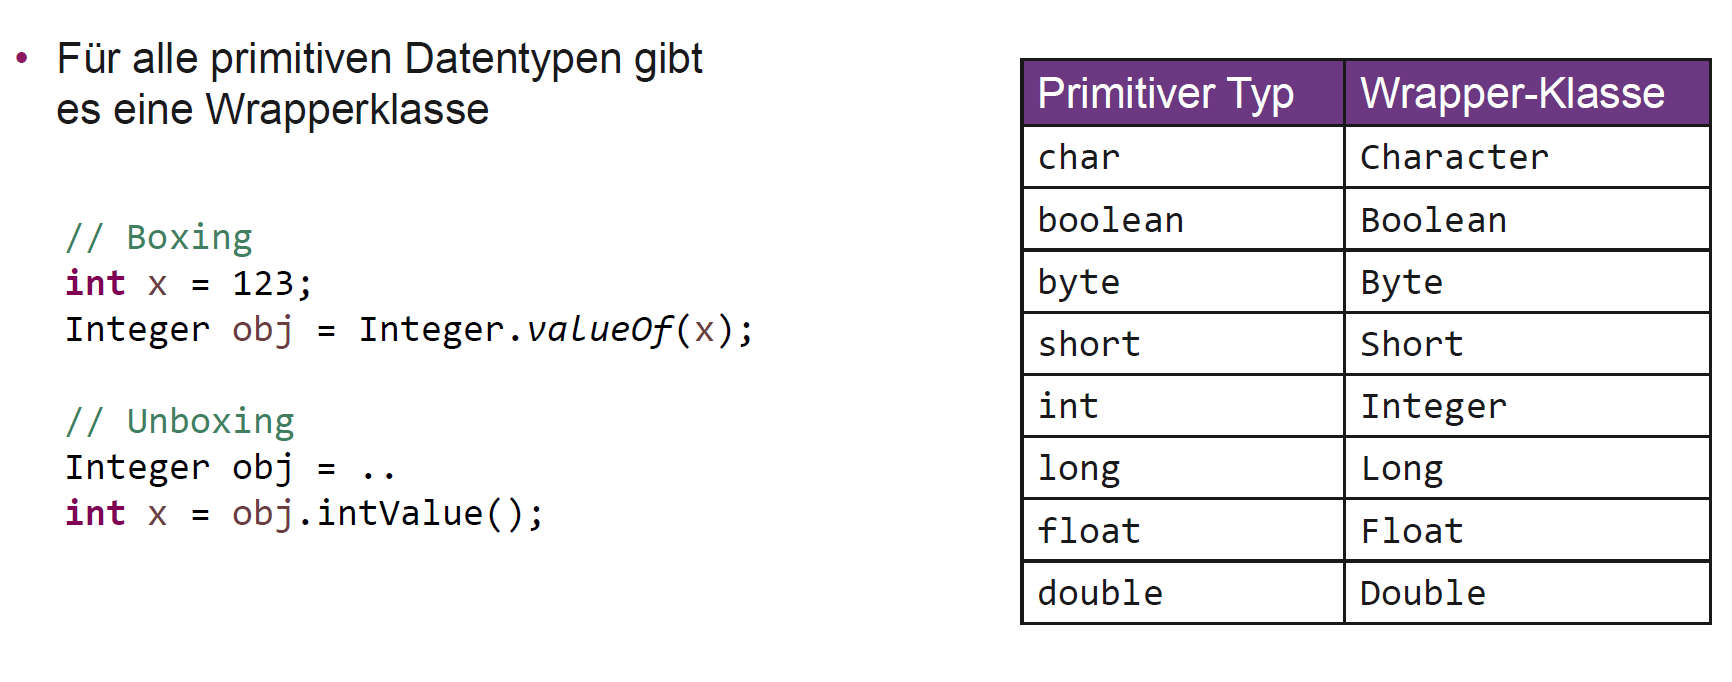
\includegraphics[width=0.9\columnwidth]{pictures/wrapper-klassen.png}
\end{center}

\subsection{ArrayList}
ArrayLists sind eine geordnete Folge von Elementen mit demselben Referenzdatentyp. Elemente können einfach 
hinzugefügt oder entfernt werden.\\
Der Zugriff auf Elemente erfolgt über Index (0 ... size()-1). Die Liste verwendet intern ein Array zur Verwaltung der Elemente.
Zu Beginn enthält sie, sofern nicht anders definiert, 10 Elemente und wird bei Erreichen der Kapazität mit Faktor 1.5 mulitpliziert.

\begin{center}
    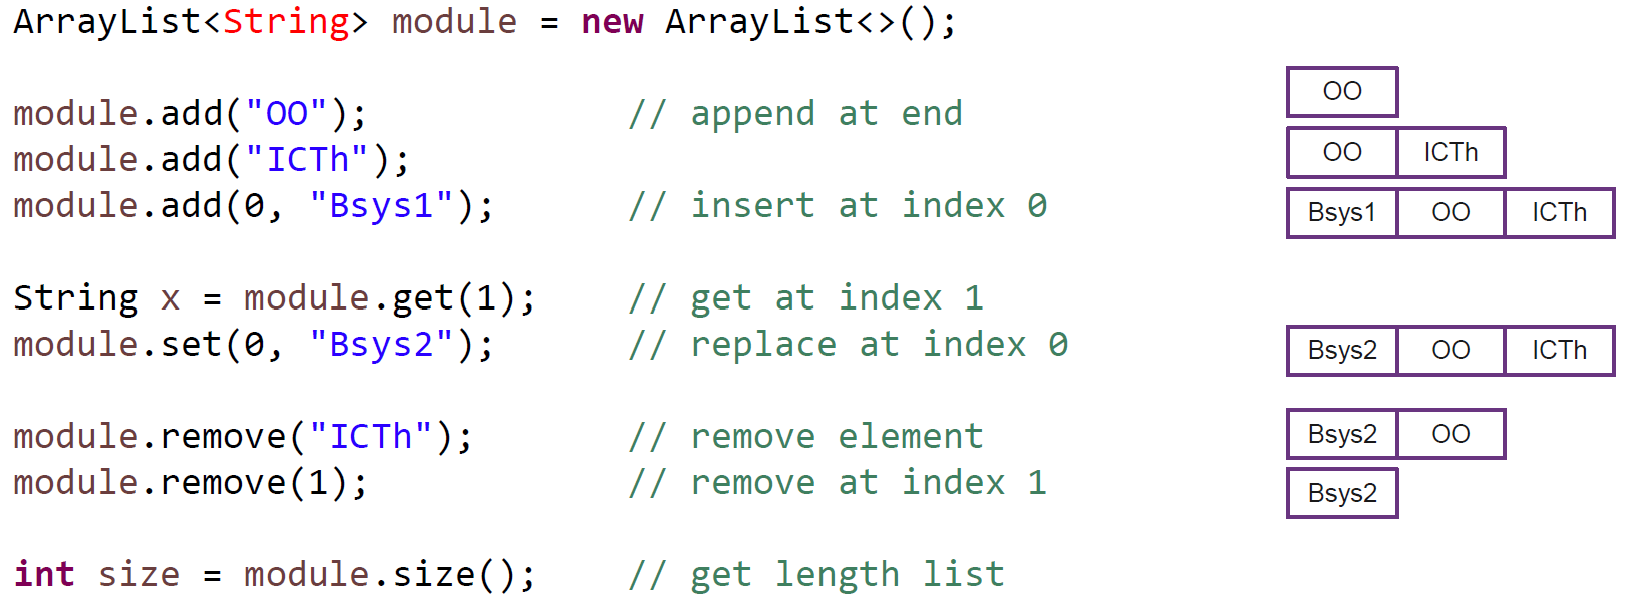
\includegraphics[width=0.9\columnwidth]{pictures/arrayList-bsp.png}
\end{center}

\begin{center}
    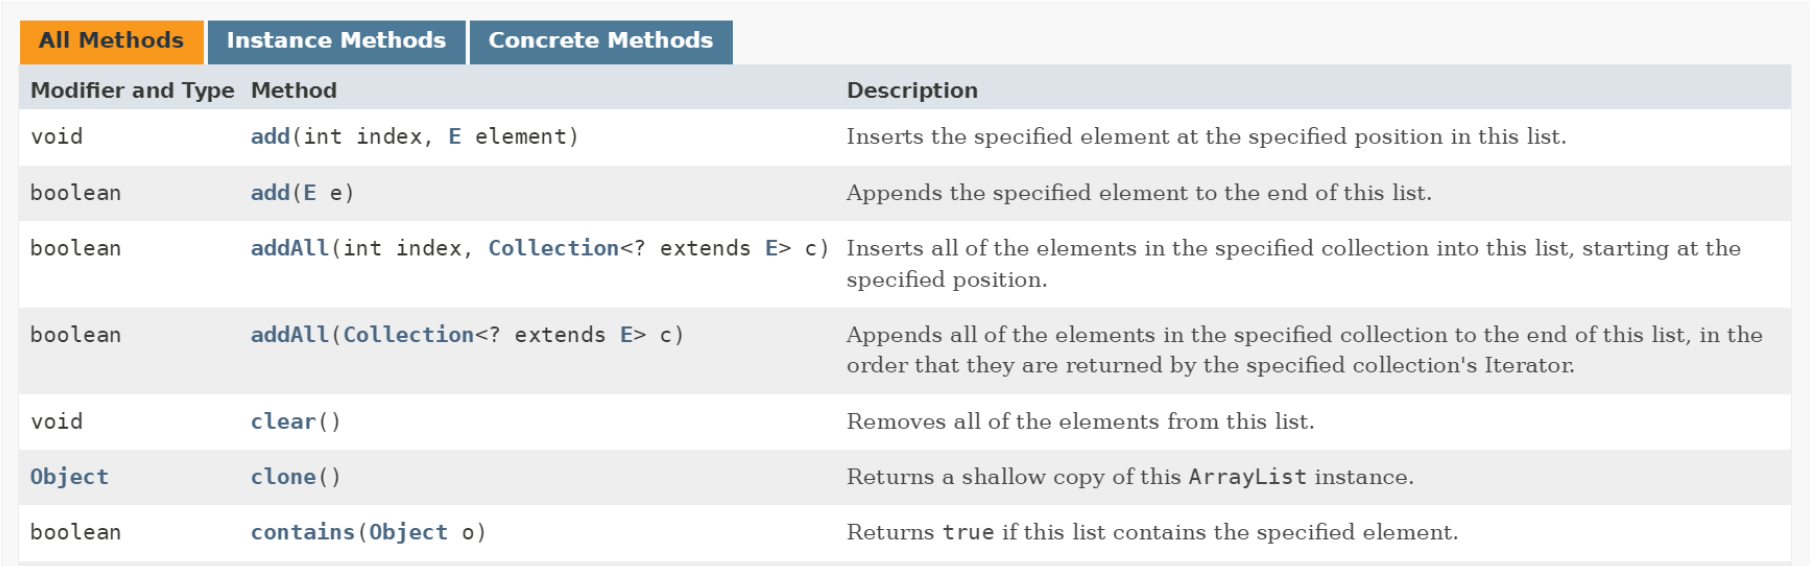
\includegraphics[width=0.9\columnwidth]{pictures/arrayList-api.png}
\end{center}

\subsection{LinkedList}
Funktioniert ähnlich wie ArrayList. Die Implementierungerfolgt mit einer doppelt-verketteten Liste.
Ausschlaggebend ist das schnelle Einfügen am Anfang oder Ende der Liste.

\subsection{HashSet}

\subsection{TreeSet}

\subsection{HashMap}

\subsection{TreeMap}

\section{Vererbung}
Die Vererbung funktioniert in Java ähnlich wie in C++. Eine Klasse in Java kann jedoch nur \textbf{eine} Basisklasse haben.
Eine abgeleitete Klasse erbt die Instanzvariablen und Instanzmethoden der Basisklasse.
Die oberste Klasse aller Basisklassen ist \verb|Object|. Methoden von \verb|Object| sind:
\begin{itemize}
    \item \verb|public String toString()|
    \item \verb|public boolean equals(Object obj)|
    \item \verb|public int hashCode()|
    \item ...
\end{itemize}

\subsection{Impliziter Code in Vererbung}
\begin{center}
    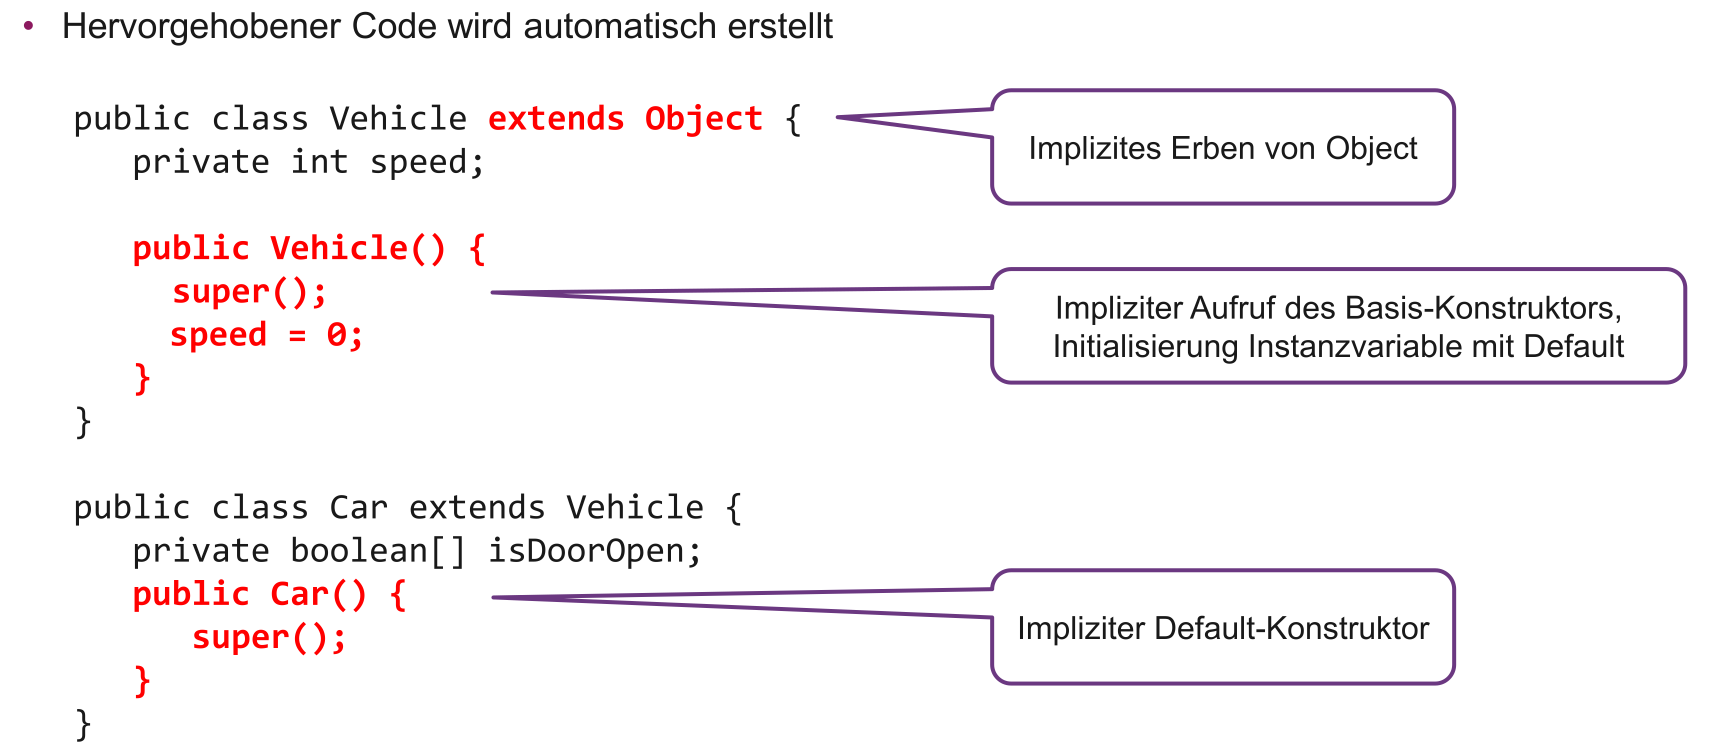
\includegraphics[width=0.9\columnwidth]{pictures/vererbung-implizit.png}
\end{center}

\subsection{Konstruktor bei Vererbung}
\begin{center}
    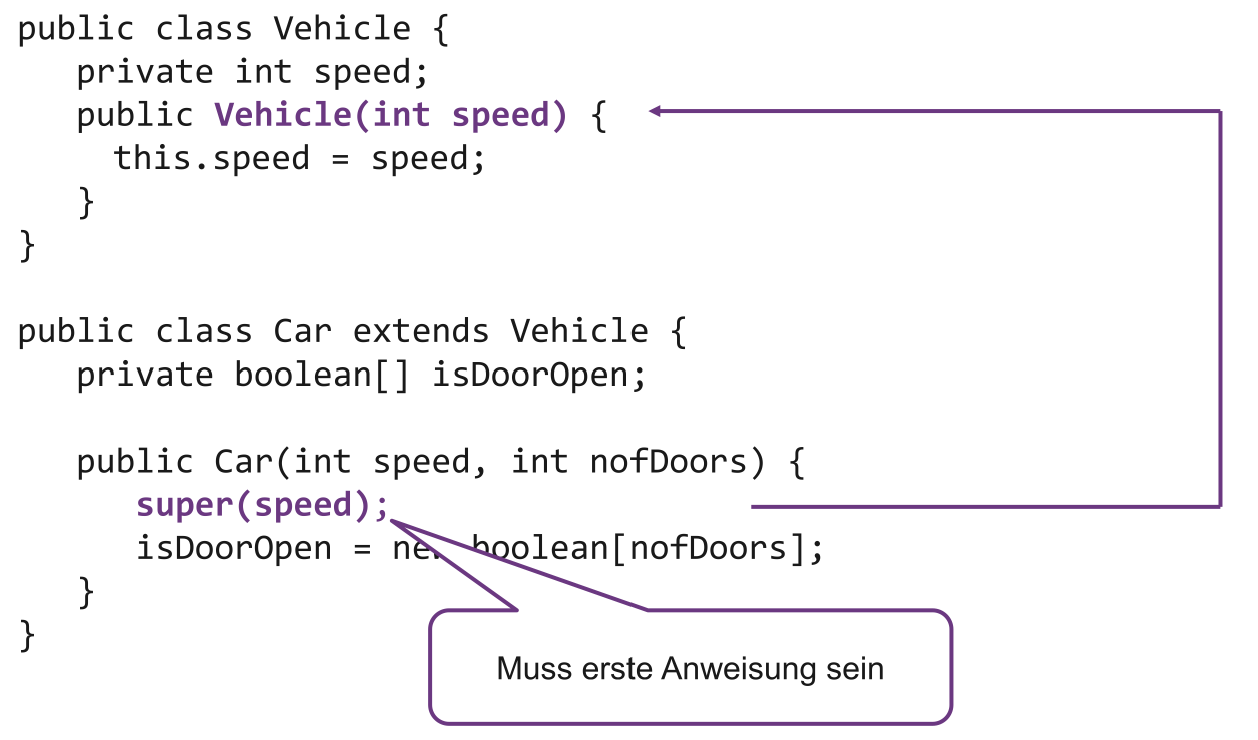
\includegraphics[width=0.9\columnwidth]{pictures/vererbung-konstr.png}
\end{center}

\subsection{Overriden von Methoden}
Gleiche Funktion wie das Keyword \verb|virtual| in C++, dieses gibt es jedoch nicht in Java. Stattdessen wird
vor einer neu implementierten Methode einer Subklasse das Schlüsselwort \verb|@Override| gesetzt. Dies ist optional, aber sinnvoll.\\
\verb|@Override|\\
\verb|public void print()|\\

Mit \verb|super| wir eine überschriebene Methode aufgerufen.
\begin{center}
    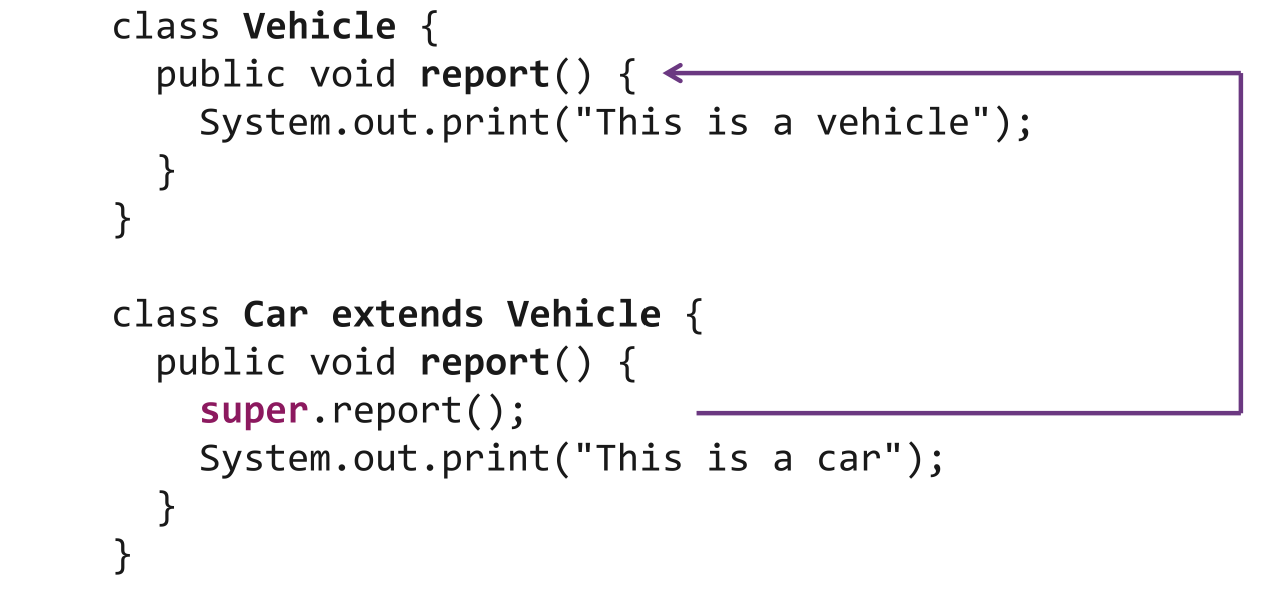
\includegraphics[width=0.9\columnwidth]{pictures/super.png}
\end{center}

\subsection{Abstrakte Klassen}
Schlüsselwort: \verb|abstract|\\

Eine abstrakte Klasse ist nicht vollständig implementiert, sprich einzelne Methoden können nicht implementiert 
sein und die Klasse kann nicht instanziiert werden.

Sie dient als Basistyp für Sub-Klassen (statischer Typ) und vererbt ihre Grundfunktionalität an Sub-Klassen.\\
Beispiel:\\
\begin{minipage}{0.5\columnwidth}
    \begin{center}
        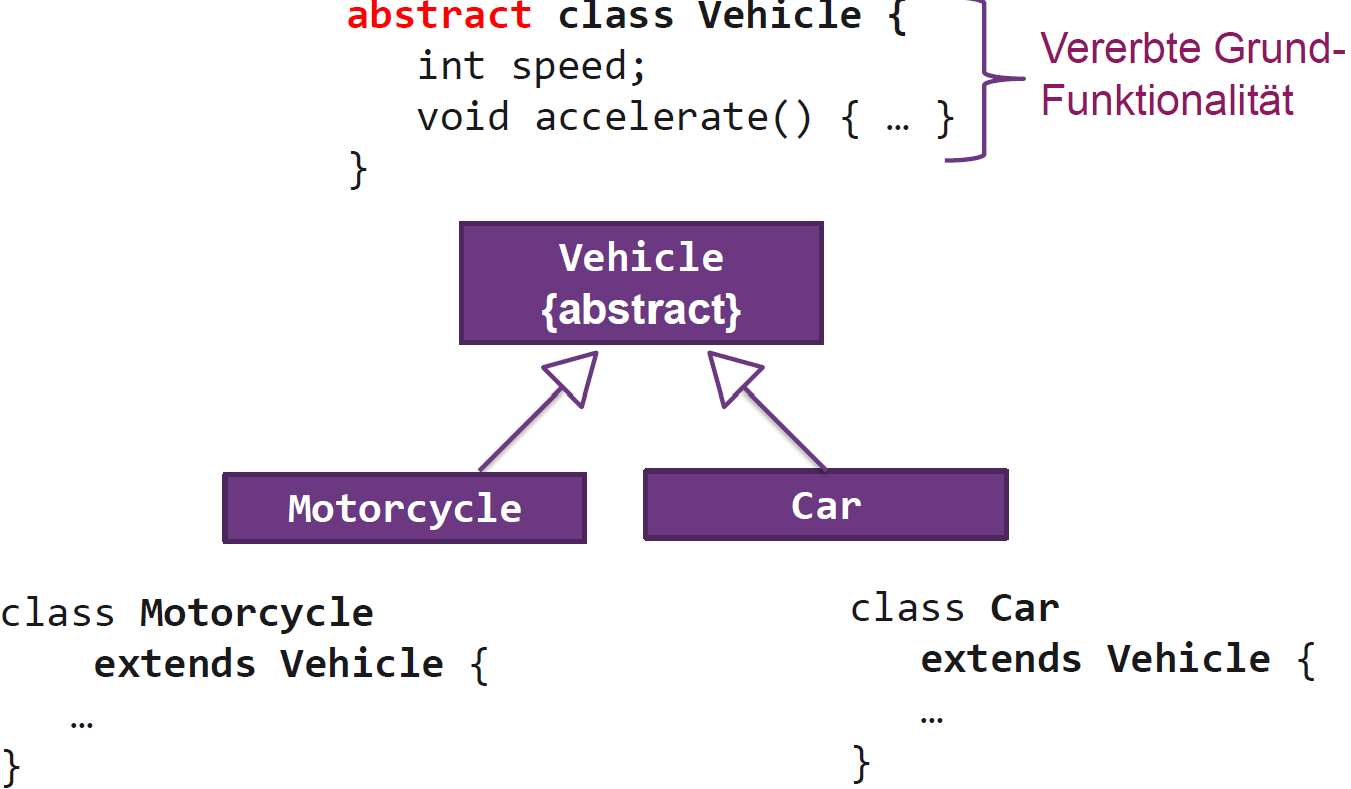
\includegraphics[width=0.9\columnwidth]{pictures/abstrakte-Klasse-Bsp.png}
    \end{center}
\end{minipage}
\hfill
\begin{minipage}{0.5\columnwidth}
    \begin{center}
        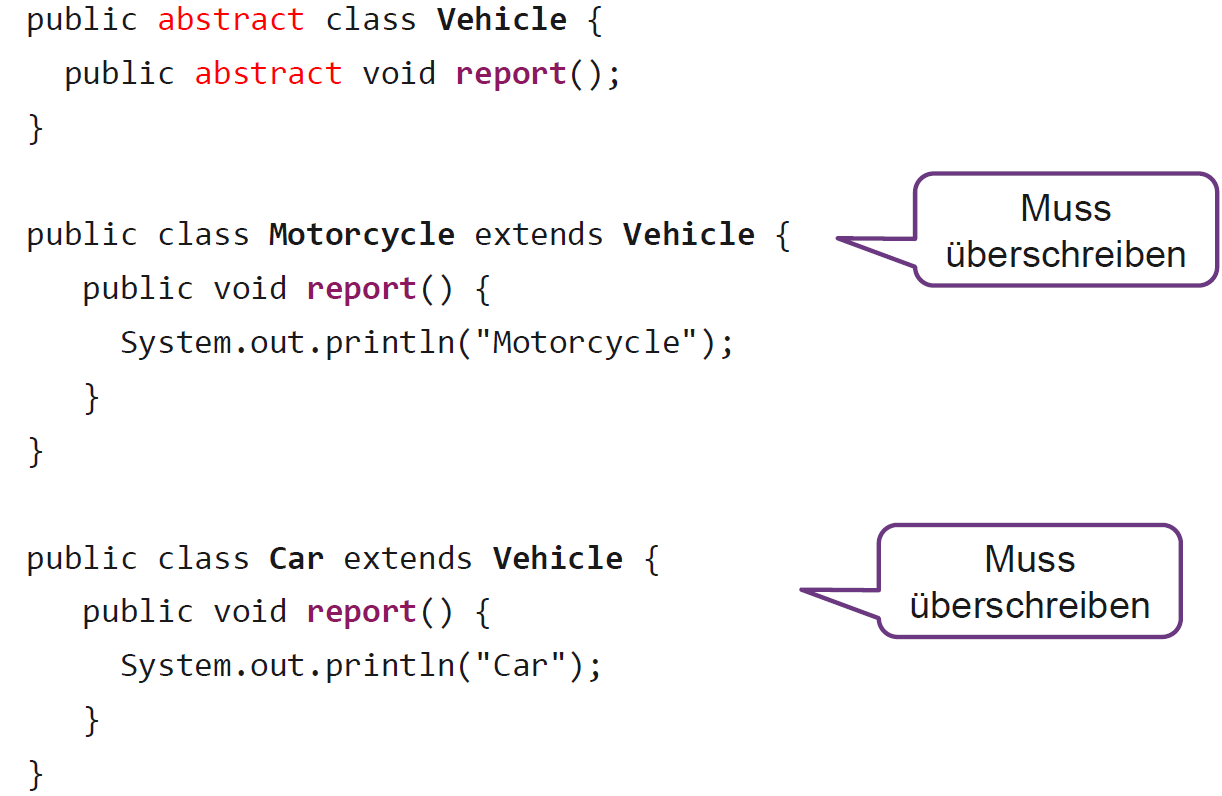
\includegraphics[width=0.9\columnwidth]{pictures/abstrakte-Klasse-Bsp2.png}
    \end{center}
\end{minipage}

\section{Binding}
\subsection{Dynamic Binding}
Generell bei nicht-privaten Instanzmethoden

\subsection{Static Binding}
Generell bei privaten Instanzmethoden (In Subklasse nicht mehr sichtbar $\rightarrow$ Neudef. der Methode) und statischen Methoden